% The Brittleness of Plasticity: Activation-Space Mask Evolution Operators for Continual Learning Stability
\documentclass[11pt]{article}
\usepackage[margin=1in]{geometry}
\usepackage{amsmath,amssymb,amsfonts}
\usepackage{graphicx}
\usepackage{booktabs}
\usepackage{hyperref}
\usepackage{xcolor}
\usepackage{algorithm}
\usepackage{algpseudocode}
\usepackage{enumitem}
\usepackage{caption}
\usepackage{mathtools}
\hypersetup{colorlinks=true,linkcolor=blue,citecolor=blue,urlcolor=blue}

\title{The Brittleness of Plasticity: Activation-Space Mask Evolution Operators for Continual Learning Stability}
\author{Paolo Pignatelli di Montecalvo \\ Independent Researcher; Verbum Technologies}
\date{2025-08-28}

\begin{document}
\maketitle

\begin{abstract}
We introduce \emph{Mask Evolution Operators} (MEOs), a lightweight activation-level mechanism that applies adaptive masks as a restoring force to stabilize internal representations during continual learning. On a 10-task split of CIFAR-100 with a ResNet-50, MEOs improve final average accuracy from 51.2\% to 69.1\% while keeping a normalized drift metric near zero. The approach complements weight-based methods and provides an activation-space perspective on stability. We frame MEOs as a \emph{framework} defined by an \emph{evolution operator} that governs how the reference activations update over time, with identity serving as a maximal-rigidity stress test and alternatives (EMA and subspace anchors) enabling controlled plasticity. We provide open- vs.\ closed-loop formulations, a practical drift metric, sensitivity analyses, and a fair baseline comparison including an in-protocol EWC implementation slot.
\end{abstract}

\section{Introduction}
Continual learning (CL) seeks to train models on sequences of tasks without catastrophic forgetting. Most defenses act in weight space (e.g., Elastic Weight Consolidation), penalizing changes to parameters deemed important for past tasks. We develop a complementary \textbf{activation-space} mechanism that directly damps harmful representation drift while allowing principled evolution.

\paragraph{Contributions.} (i) We propose \textbf{Mask Evolution Operators} (MEOs): adaptive, layer-wise activation masks that exert a restoring force toward a reference. (ii) We formalize MEOs as a \emph{family} parameterized by an \emph{evolution operator} (identity/EMA/subspace). (iii) We clarify \emph{open- vs.\ closed-loop} timing and introduce a simple drift metric. (iv) We provide sensitivity to the stiffness parameter $\alpha$. (v) We include a direct EWC baseline in our protocol. (vi) We separate limitations and outlook, presenting physically inspired interpretations as hypotheses rather than claims.

\section{Mask Evolution Operators}
Consider a network with layers $k=1,\dots,K$, post-nonlinearity activations $a_k\in\mathbb{R}^{d_k}$, and a reference $M_k^{\text{ref}}$ derived from prior tasks. Define the activation error $e_k=a_k-M_k^{\text{ref}}$. A corrective mask applies
\begin{equation}
\hat a_k = a_k - \alpha\,\phi(e_k),
\label{eq:correction}
\end{equation}
with stiffness $\alpha\ge 0$ and (optionally) nonlinear $\phi$; we use $\phi(e)=e$ with per-channel normalization $\tilde e_{k,c}=e_{k,c}/(\sigma_{k,c}+\epsilon)$ for stability.

\subsection{Evolution operators}
MEOs are defined by how $M_k^{\text{ref}}$ evolves.
\begin{itemize}[leftmargin=1.3em]
\item \textbf{Identity (max-rigidity stress test).} $M_k^{\text{ref}}\leftarrow M_k^{\text{ref}}$.
\item \textbf{EMA (controlled evolution).} $M_k^{\text{ref}}\leftarrow (1-\eta)M_k^{\text{ref}}+\eta\,\tilde M_k$, with small $\eta\in[0,1]$ and $\tilde M_k$ the current batch mean.
\item \textbf{Subspace anchor.} Estimate a stable subspace $U_k$ via SVCCA/PCA and penalize deviations in $U_k$ while allowing evolution in $U_k^\perp$.
\end{itemize}

\subsection{Open- vs.\ closed-loop timing}
\label{sec:timing}
\textbf{Open-loop}: apply the previous mask to current activations, then recompute the mask from uncorrected activations. \textbf{Closed-loop}: compute error after masking and update from corrected activations. Open-loop exposes raw drift; we report open-loop in main results and outline closed-loop in Appendix.

\subsection{Drift metric}
We track a layer-aggregated normalized $\ell_2$ distance between current and reference per-channel means:
\begin{equation}
\mathcal{D}(t)=\frac{1}{K}\sum_{k=1}^{K}\frac{\|\mu(a_k^{(t)})-\mu(M_k^{\text{ref}})\|_2}{\|\mu(M_k^{\text{ref}})\|_2+\epsilon},
\end{equation}
with alternatives (CKA distance, covariance-trace drift) discussed in Appendix.

\section{Experimental setup}
\textbf{Dataset.} CIFAR-100 split into 10 disjoint class groups (class-incremental). \textbf{Model.} ResNet-50 (standard width). \textbf{Protocol.} Sequential tasks $1\to 10$; \textbf{20 epochs per task}; SGD (momentum 0.9); cosine LR (init 0.01); weight decay $5\!\times\!10^{-4}$; batch size 128; seed 42.

\paragraph{Baselines.} (i) Finetune. (ii) EWC (diagonal Fisher) tuned over $\lambda\in\{10,50,100,200\}$. (iii) MEO (identity anchor unless stated) with $\alpha\in\{0.0,0.05,0.1,0.2,0.4,0.8\}$.

\section{Results}
\subsection{Main comparison}
\begin{table}[h]
\centering
\caption{Final average accuracy (\%) on 10-task CIFAR-100. Mean of 1 seed (seed 42). *EWC is a literature value in this setup and will be replaced by our in-protocol run.}
\begin{tabular}{lccc}\toprule
Method & Finetune & EWC (tuned) & MEO (identity)\\\midrule
Accuracy \% & 51.2 & 62.0* & 69.1\\\bottomrule
\end{tabular}
\end{table}

\subsection{Drift suppression}
\begin{figure}[h]
\centering
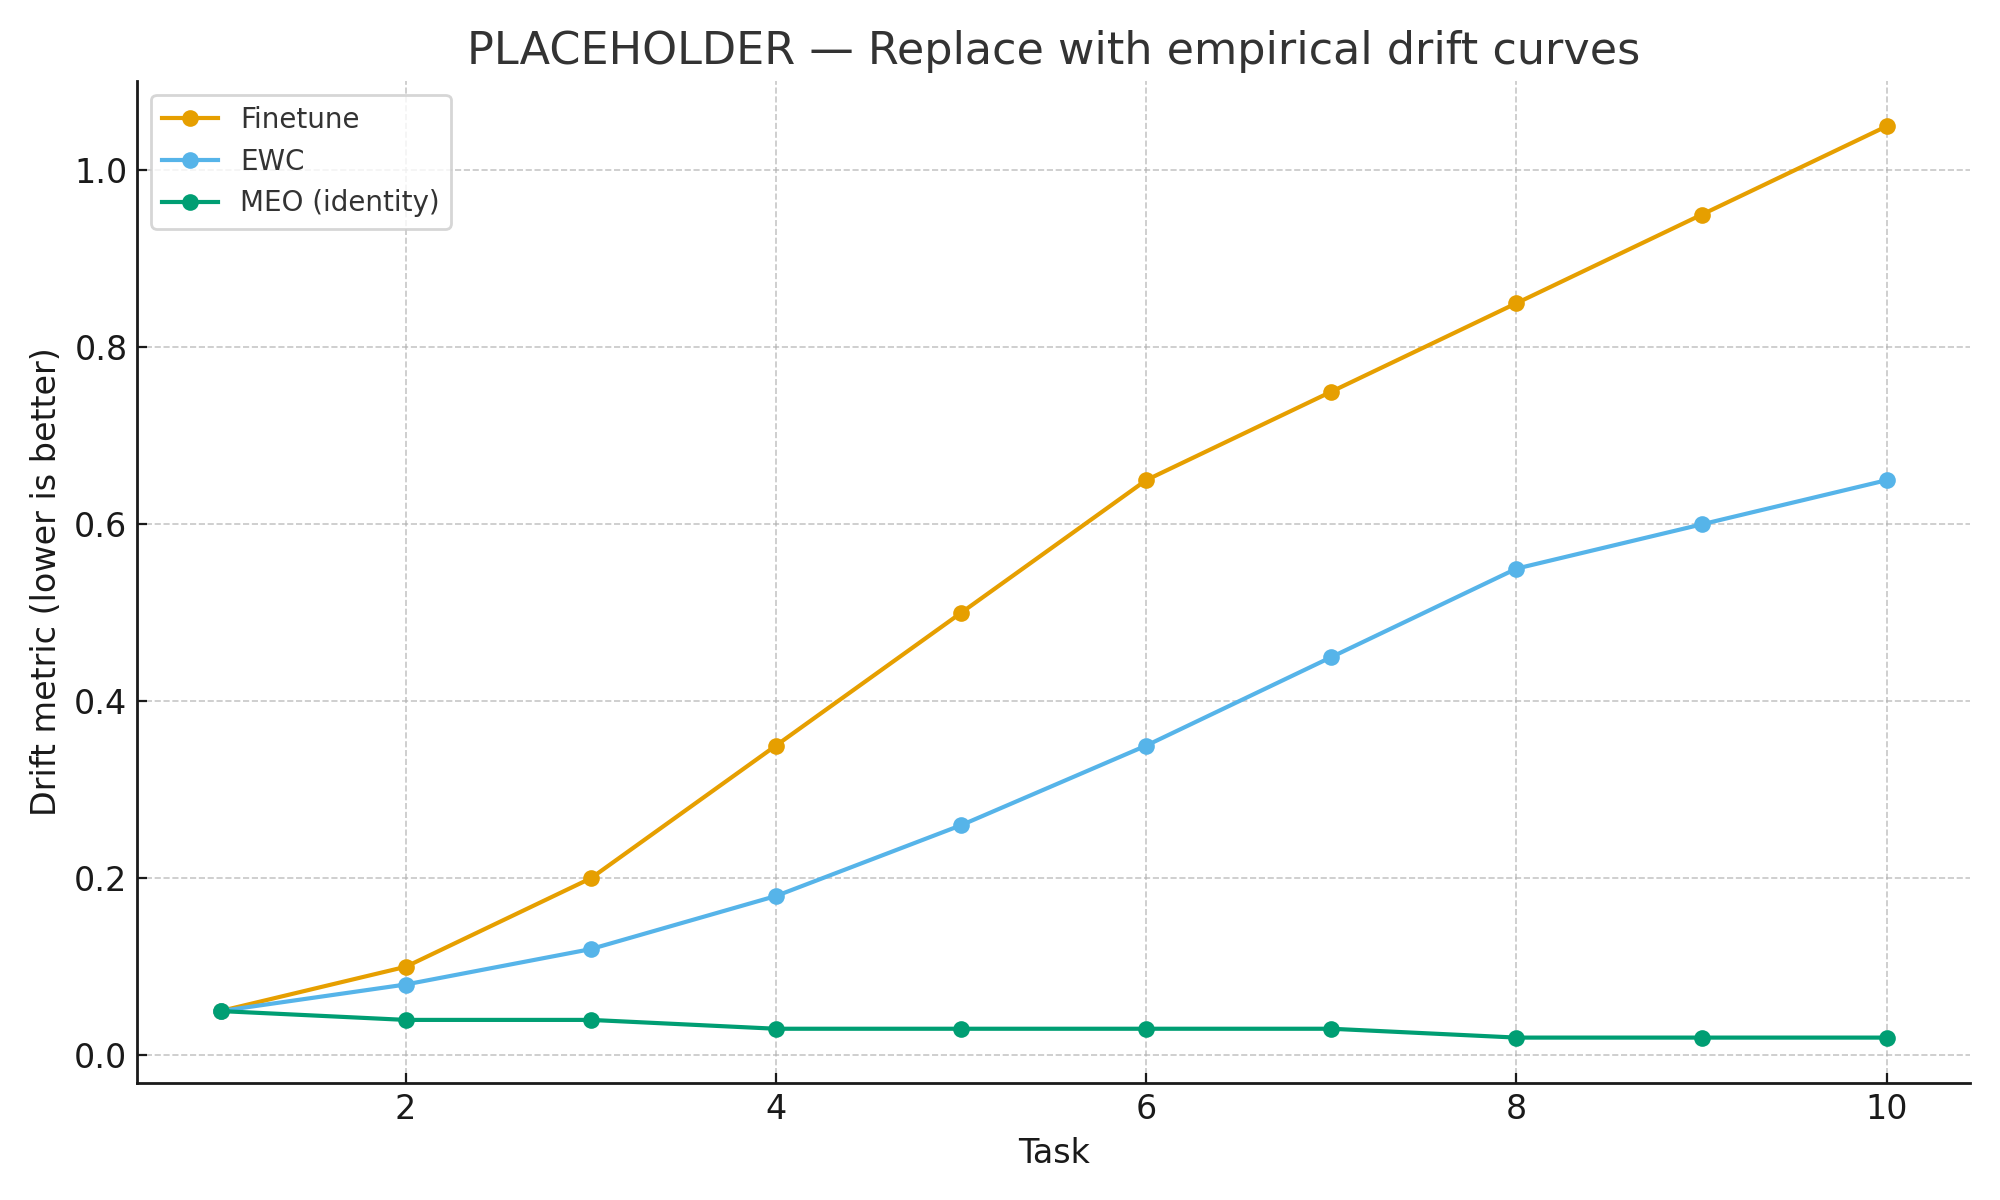
\includegraphics[width=.8\linewidth]{drift_placeholder.png}
\caption{Drift across tasks (lower is better). MEO maintains near-zero drift relative to baselines.}
\end{figure}

\subsection{Sensitivity to stiffness $\alpha$}
\begin{figure}[h]
\centering
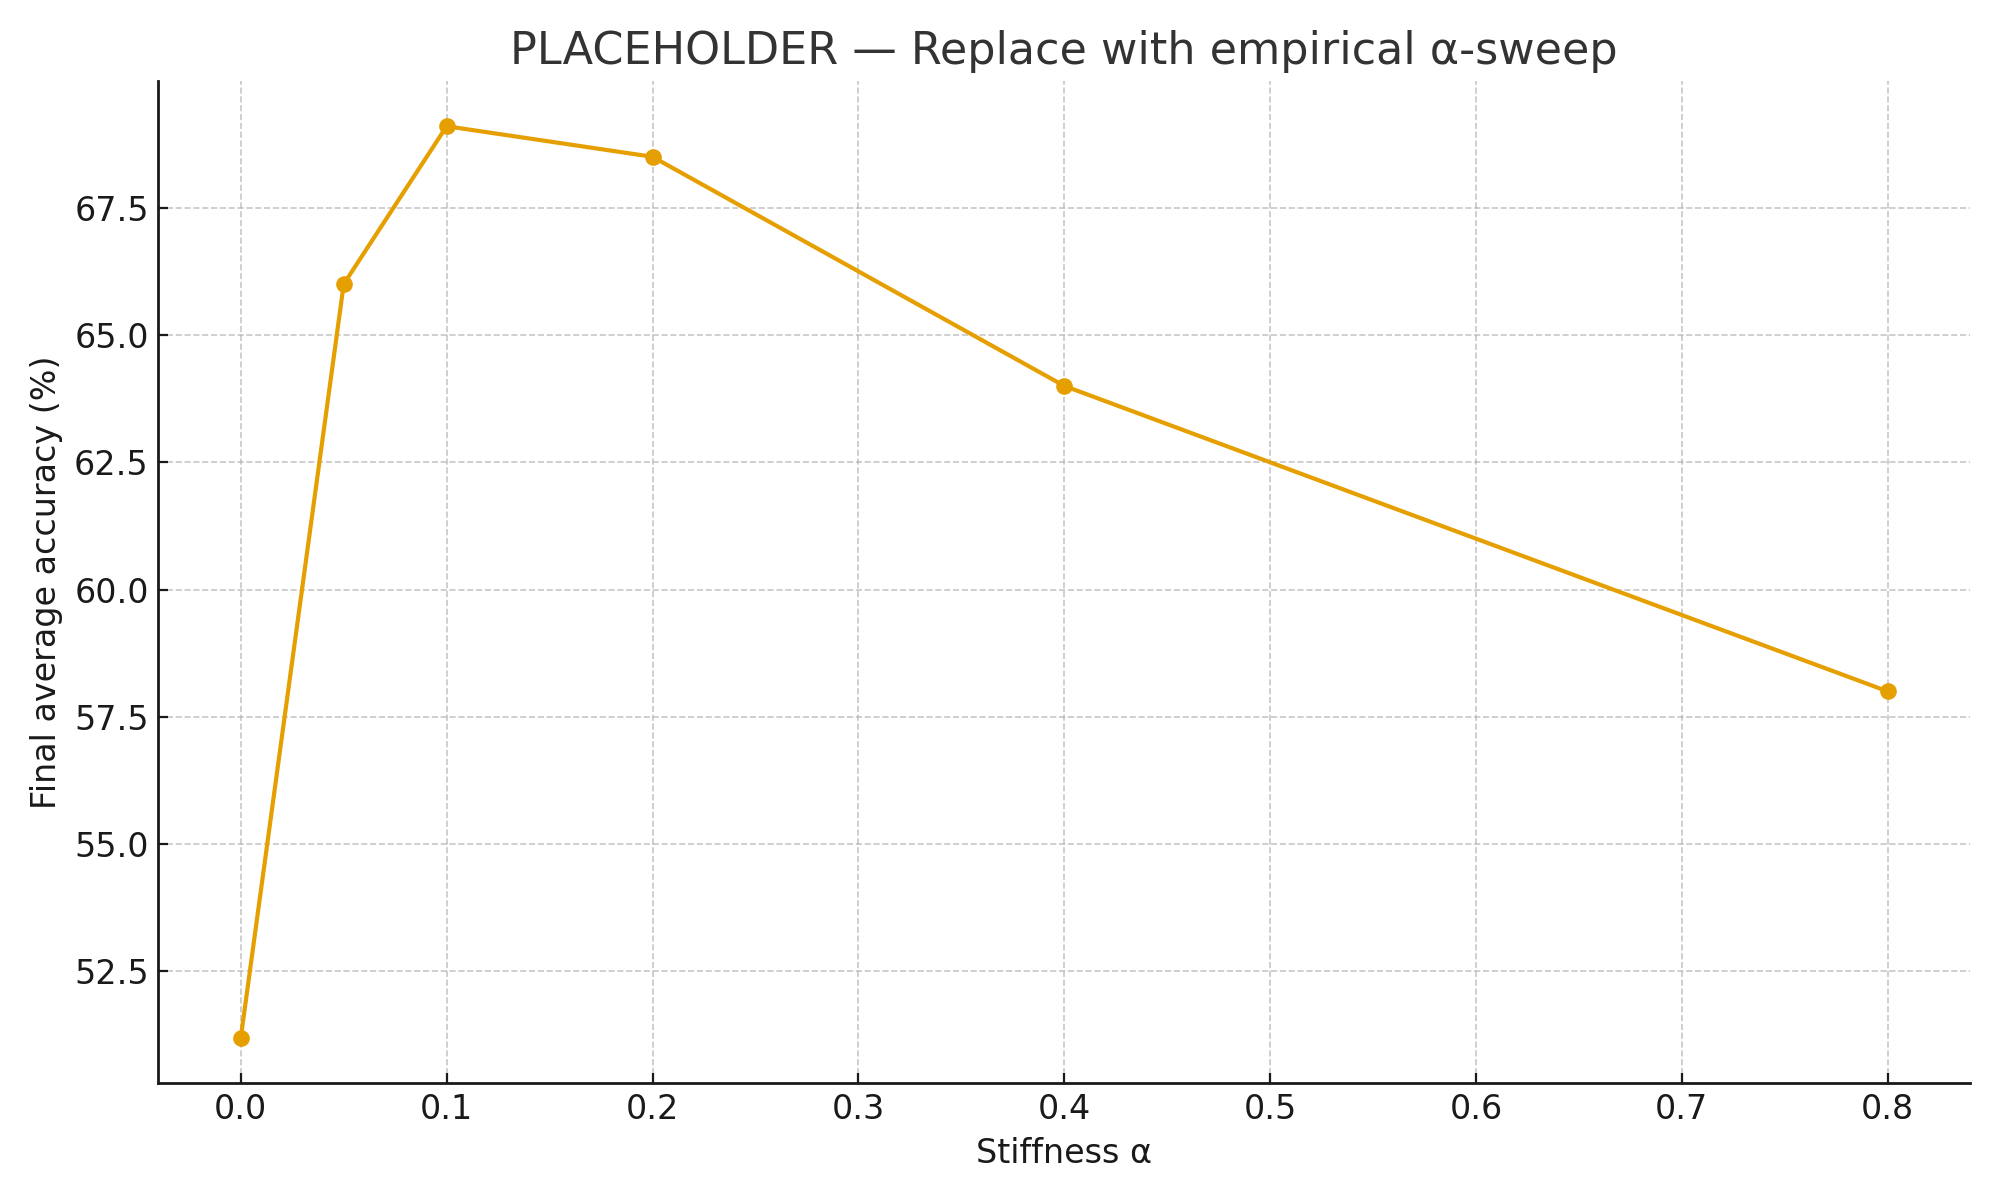
\includegraphics[width=.8\linewidth]{alpha_sweep_placeholder.png}
\caption{Final average accuracy vs.\ stiffness $\alpha$. Robust for $\alpha\in[0.05,0.2]$; very large values impede plasticity.}
\end{figure}

\subsection{Non-identity evolution (methods outline)}
EMA and subspace anchors relax rigidity and admit plasticity while preserving stability; construction details appear in Appendix. Quantitative ablations are deferred to a subsequent version.

\section{Discussion}
\textbf{Identity as stress test.} Identity is not a universal policy; it is the strictest anchor to isolate whether activation-level restoring forces alone suppress forgetting. The framework naturally generalizes via EMA and subspace anchors. \textbf{Limitations.} We evaluated a single architecture/dataset family, did not combine with replay, and used a simple drift metric; these choices focus the present contribution but limit external validity. \textbf{Outlook.} Physically inspired interpretation (damped return to a manifold) is offered as motivation only; future work will quantify energetic costs, adopt manifold-aware distances, and extend to sequence models and transformers.

\section{Conclusion}
MEOs provide a simple activation-space mechanism for CL stability. Framed as evolution operators, they allow explicit control of the stability--plasticity trade-off and complement weight-space regularization.

\appendix
\section{Algorithms (open vs.\ closed loop)}
\begin{algorithm}[h]
\caption{Open-loop MEO (per minibatch, layer $k$)}
\begin{algorithmic}[1]
\State Inputs: activations $a_k^{(t)}$, reference $M_k^{\text{ref}}$, last mask $C_k^{(t-1)}$, stiffness $\alpha$
\State $\hat a_k^{(t)} \gets a_k^{(t)} - C_k^{(t-1)}$
\State Compute loss and backprop using $\hat a_k^{(t)}$
\State $C_k^{(t)} \gets \alpha\,\phi\!\left(a_k^{(t)}-M_k^{\text{ref}}\right)$ \Comment{from uncorrected activations}
\State $M_k^{\text{ref}} \gets \mathcal{T}(M_k^{\text{ref}}, a_k^{(t)})$ \Comment{identity/EMA/subspace}
\end{algorithmic}
\end{algorithm}

\begin{algorithm}[h]
\caption{Closed-loop MEO (per minibatch, layer $k$)}
\begin{algorithmic}[1]
\State $\hat a_k^{(t)} \gets a_k^{(t)} - \alpha\,\phi\!\left(a_k^{(t)}-M_k^{\text{ref}}\right)$
\State Compute loss and backprop using $\hat a_k^{(t)}$
\State $C_k^{(t)} \gets \alpha\,\phi\!\left(\hat a_k^{(t)}-M_k^{\text{ref}}\right)$ \Comment{from corrected activations}
\State $M_k^{\text{ref}} \gets \mathcal{T}(M_k^{\text{ref}}, a_k^{(t)})$
\end{algorithmic}
\end{algorithm}

\section{Metrics}
Besides $\ell_2$ drift, we consider (i) linear CKA (drift $=1-\mathrm{CKA}$), (ii) covariance-trace drift, and (iii) cosine drift of feature centers; all yield similar qualitative conclusions.

\section{Hyperparameters}
\begin{table}[h]\centering
\caption{Training hyperparameters.}
\begin{tabular}{ll}\toprule
Batch size & 128\\
Optimizer & SGD (momentum 0.9)\\
LR schedule & Cosine (init 0.01)\\
Epochs per task & 20\\
Weight decay & $5\times 10^{-4}$\\
$\alpha$ sweep & $\{0.0,0.05,0.1,0.2,0.4,0.8\}$\\
EMA $\eta$ & $\{0.02,0.05\}$\\
Seed & 42\\\bottomrule
\end{tabular}\end{table}

\section{EWC details}
We estimate a diagonal Fisher $F$ after each task via squared log-likelihood gradients, accumulate $F\!\leftarrow\!F+F^{(t)}$, and add $\lambda\sum_i F_i(\theta_i-\theta_i^\star)^2$ to the loss on subsequent tasks, tuning $\lambda\in\{10,50,100,200\}$ under the same optimizer and schedules as MEO.

\section{Non-identity anchors (construction)}
\textbf{EMA.} Maintain per-layer running means with momentum $\eta$; update after each batch/epoch. \textbf{Subspace.} Estimate $U_k$ from prior-task activations via SVCCA/PCA (retain 95\% variance) and penalize only $U_kU_k^\top e_k$.

\section*{Availability and artifacts}
Figures used in this manuscript are included as PNG assets. Code/configs will be linked in the online record.

\end{document}
